\chapter{Background}
\label{ch:cs}
In this chapter, we will introduce the theory of \emph{Compressive Sensing} (also known as \emph{Compressed Sensing, Compressive Sampling} or simply, \emph{CS}).
CS is a framework within signal processing that allows for acquiring signals (i.e. measure or \emph{sense}) directly in a \emph{compressed} format.

To motivate the discussion, we will first review the conventional approach to signal acquisition and compression.

\section{Coventional Signal Processing}
\subsection{Signal Acquisition}
In order to work with information within analog signals (continuous streams of data) such as sounds, images or video, we rely on reducing the analog signals to digital (discrete) signals that can be processed with computers.
This digitization is done by taking discrete measurements of the analog signal at certain points in time or space, a process known as \emph{sampling}.

Conventional approaches to sampling are based on the \emph{Shannon/Nyquist Sampling Theorem} \cite{shannon1949}:
When sampling a signal uniformly, we are able to \emph{perfectly reconstruct} the signal from its samples if the sampling rate is at least twice the highest frequency present in the signal.

Consider an analog signal $x(t)$ that varies with time, such as an audio wave.
Let $f$ be the highest frequency present in $x(t)$.

In order to digitise $x(t)$, we measure $x$ at discrete points in time $t^{(0)}, \cdots, t^{(n)}$ and store the samples $x^{(i)} \equiv x(t^{(i)})$.
We sample $x$ uniformly, measuring a sample every $T_s$ seconds, so that $t^{(i)} = iT_s$.
The sampling rate is therefore $f_s = 1/T_s$.

\begin{figure}
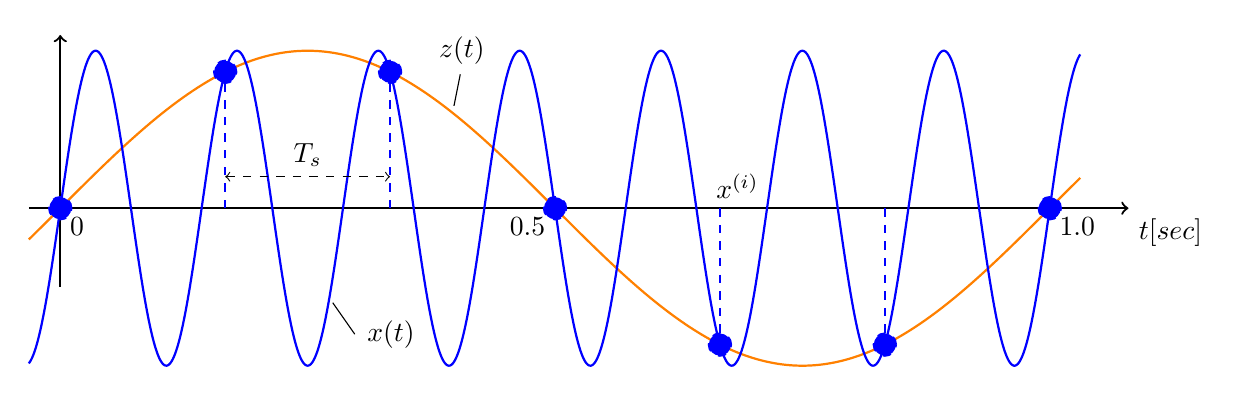
\begin{tikzpicture}[scale=2]
  \draw [thick,->](-0.2,0) -- (2*pi+0.5,0) node[below right] {$t [sec]$};
  \draw [thick,->](0,-0.5) -- (0,1.1);
  \draw [domain=-0.2:2*pi+0.2,samples=1000,orange, thick] plot(\x,{sin(\x r)});
  \draw [domain=-0.2:2*pi+0.2,samples=1000,blue, thick] plot(\x,{sin(7*\x r)});  
  \draw [domain=0:2*pi, samples=7, ycomb, mark=*,blue, dashed, thick] plot(\x,{sin(\x r)});
  \node at (2.55,1) {$z(t)$};
  \draw (2.54,0.85) -- (2.5,0.65);
  \node at (2.1,-0.8) {$x(t)$};
  \draw (1.87,-0.8) -- (1.73,-0.6);
  \node at (4.3,0) [above] {$x^{(i)}$};
  \node at (2*pi,0) [below right] {$1.0$};
  \node at (pi,0) [below left] {$0.5$};
  \node at (0,0) [below right] {$0$};
  \draw [<->, thin, dashed] (pi/3,0.2) -- (pi/2,0.2) node[above] {$T_s$} --(2*pi/3,0.2);
\end{tikzpicture}
\caption[Illustration of Nyquist Sampling]{Illustration of the Shannon/Nyquist Sampling Theorem. The blue curve is the original signal $x(t)$ which is a sinusoid with frequency $f = 7$ Hz. The blue points are discrete samples $x^{(i)}$ taken from $x(t)$ at a sampling rate $f_s = 7$ Hz, which is below the Nyquist Rate $2f = 14$ Hz. Thus, aliasing occurs and interpolation algorithms will reconstruct an alias $z(t)$ (orange curve) of $x(t)$.}
\label{fig:nyquist}
\end{figure}

Suppose we wish to reconstruct $x(t)$ by interpolating the samples.
There is an infinite number of continuous functions that fit this set of samples.
However, it can be shown that only one of them has a bandwidth of no more than $f_s/2$.
Thus, if $f < f_s/2$ (the \emph{Nyquist Criterion}), then $x(t)$ is the unique function that will be approximated by interpolation algorithms such as the \emph{Whittaker-Shannon interpolation formula} \cite{shannon1949}.

In Figure \ref{fig:nyquist}, we have a sinusoidal signal $x(t)$ with frequency $f$.
The sampling rate is $f_s=f$ and therefore below the signal's \emph{Nyquist rate} $2f$. 
Thus, we are unable to reconstruct $x(t)$ from the samples. 
Instead, we will reconstruct an \emph{alias} $z(t)$ which, in this case, is another sinusoid with frequency $f/7$.
The original signal $x$ is lost.

We have illustrated Nyquist sampling in the 1-dimensional case.
The same principles hold for higher dimensional signals such as images and videos.

For signals that vary with space, the sampling rate is governed by the desired spatial resolution.
In order to recover the finer details (the high-frequency components) of an image, we require a higher pixel density (i.e. a larger number of pixels per centimeter (ppcm)).

Nyquist sampling underlies almost all signal acquisition protocols that are found in practice. 
It is the basis of medical imaging, audio and video recording and radio receivers.

\subsection{Signal Compression}
\label{sect:compression}
The sampling theorem imposes a lower bound on the sampling rate above which we are able to perfectly reconstruct the desired signal.
This lower bound is often very high and we end up with a very large number of measurements.
Storage and transfer of such signals becomes prohibitively expensive as the size of the signal grows.
Thus, a need for \emph{data compression} arises.

We will discuss a particular type compression algorithm known as \emph{transform coding}.
It is the standard compression method for a wide range of manmade signals such as audio, photos, and video and is the basis of many common signal formats such as JPEG (images), MPEG (video) and MP3 (audio).

Let $\bm v$ by a real-valued digital signal of length $M$, $\bm v \in \mathbb{R}^M$.
Without loss of generality, $\bm v$ is assumed to be a one-dimensional signal.
If we are working with a multi-dimensional signal, we may first vectorize it into a long vector.
When compressing digital signals, we are usually interested in \emph{lossy compression}.

Any vector in $\mathbb{R}^M$ can be expressed as a linear combination of $M$ \emph{basis vectors} $\bm\psi_j \in \mathbb{R}^M$:
\begin{equation}
\label{eqn:cs-transform1}
  \bm v = \sum_{j=1}^M w_j \bm\psi_j
\end{equation}
where $w_j$ is the coefficient (or weight) associated with $\bm\psi_j$.

By forming the \emph{basis matrix} $\bm\Psi = \left[\bm\psi_1 \,\cdots\, \bm\psi_M\right]$, we can express equation (\ref{eqn:cs-transform1}) in matrix form
\begin{equation*}
\bm v = \bm\Psi \bm w
\end{equation*}
where $\bm w = (w_1,\cdots,w_M)^T$.
For simplicity, we assume that the basis $\bm\Psi$ is orthonormal, so that $\bm\Psi\bm\Psi^T = \bm I_M$ and $\bm\psi_i^T\bm\psi_j$ is 1 if $i = j$ and 0 otherwise.
Thus, the coefficient $w_j$ is given by $w_j = \bm v^T\bm\psi_j$.

We now have two equivalent representations of the same signal: $\bm v$ in the original basis and $\bm w$ in the $\bm\Psi$ basis.
Since $\bm\Psi$ is orthogonal, $\bm v$ and $\bm w$ have the same $\ell_2$-norm, $||\bm v||_2 = ||\bm\Psi\bm w||_2 = ||\bm w||_2$.
However, in the original signal, $\bm v$, the energy is typically spread over many of its components.
On the other hand, it is possible to find a basis $\bm\Psi$ such that the energy of the transformed signal, $\bm w$, is concentrated in only a few large components $w_j$ and a large fraction of its entries are very close to zero.

Suppose that we delete the entries $w_j$ that are very small and replace them with zero to obtain $\bm{\hat w}$.
Let $\bm{\hat v} = \bm\Psi\hat{\bm w}$ be the approximate signal in the original domain.
Since $\bm{\hat w}$ is very close to $\bm w$, it follows that
\begin{equation*}
  ||\bm{\hat v} - \bm v||_2 = ||\bm\Psi\bm{\hat w} - \bm\Psi\bm w||_2 = ||\bm\Psi (\bm{\hat w} - \bm w)||_2 = ||\bm{\hat w} - \bm w||_2
\end{equation*}
is very small.

\begin{figure}
  \centering
  \begin{subfigure}[b]{0.4\textwidth}
    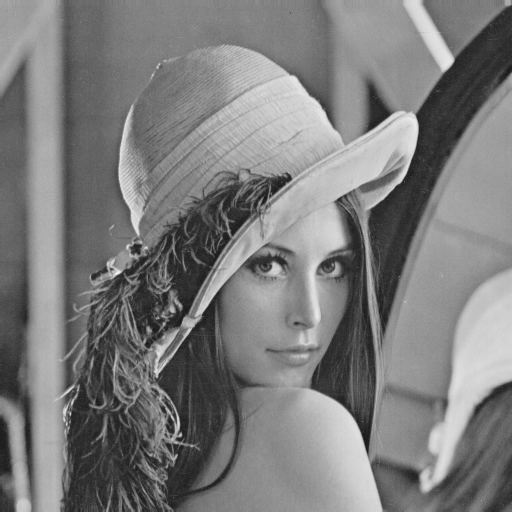
\includegraphics[width=\textwidth]{Chapter2/Images/lenna512.png}
    \caption{Uncompressed Image}
    \label{fig:ch2:lenna_orig}
  \end{subfigure}
  \begin{subfigure}[b]{0.4\textwidth}
    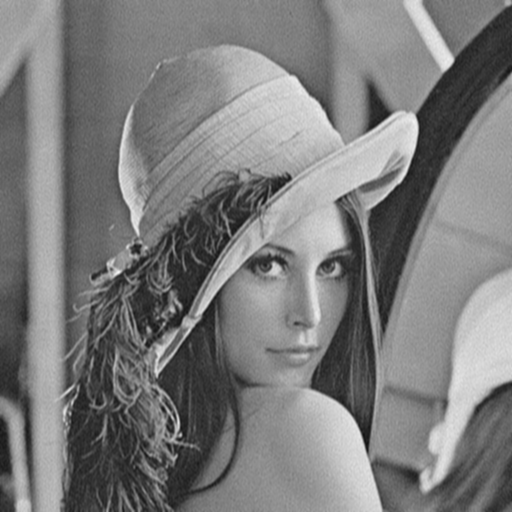
\includegraphics[width=\textwidth]{Chapter2/Images/lenna512_dct.png}
    \caption{Compressed Image via DCT}
    \label{fig:ch2:lenna_dct}
  \end{subfigure}
  \caption[Image Compression using DCT]{The uncompressed image has a resolution of $512\times 512$, i.e. 262,144 pixels. We compress the image by performing a Discrete Cosine Transform (see Section \ref{sect:dct}) and storing only the largest 27,832 coefficients. The compression ratio is 9.42.}
  \label{fig:ch2:dct}
\end{figure}

Thus, a viable method for lossy compression of the signal $\bm v \in \mathbb{R}^M$ would be the following:
\begin{enumerate}
\item Compute the full set of transform coefficients $\{w_j\}_{j=1}^M$ via $\bm w = \bm\Psi^T\bm v$.
\item Locate all the coefficients $w_j$ whose absolute value is above a certain threshold (suppose there are $K$ of them). 
\item Discard all the $(M-K)$ small coefficients
\item Store the values and locations of the $K$ large coefficients
\end{enumerate}
In order to view the compressed signal in the original domain, we reconstruct it via the transform: $\bm\Psi\bm{\hat w} = \bm{\hat v}$, where $\bm{\hat w}$ is $\bm w$ with the $(M-K)$ smallest coefficients replaced by zero.

It is possible to find basis matrices $\bm\Psi$ that result in very high compression ratios for a wide range of signals without any noticable reduction in the signal quality.
Furthermore, many of the commonly used basis transforms can be computed very efficiently.

Audio signals and a wide class of communication signals are highly compressible in the localized Fourier basis.
Images and video signals, on the other hand, can often be compressed via the \emph{Discrete Cosine Transform} (DCT) or the \emph{Discrete Wavelet Transform} (DWT).
For instance, the JPEG standard for image compression is based on the DCT \cite{wallace1992}, while the more modern JPEG2000 format uses the CDF 9/7 wavelet transform or the CDF 5/3 wavelet transform \cite{usevitch2001}.

In Figure \ref{fig:ch2:dct}, we compress the standard test image ``Lenna'' via a DCT. 
We are only storing about 10\% of the transform coefficients.
Yet, the difference between the original image and the compressed image is hardly noticable.

We will discuss the DCT and the DWT in more detail in Chapter \ref{ch:dwt}.

\section{Compressive Sensing}
The conventional approach to data acquisition and compression is very effective and has been highly influential.
However, it is also extremely wasteful.
We acquire a huge amount of data at the signal sampling stage and then proceed to discard a large part of it at the compression stage.

Compressive Sensing \cite{candes2006,donoho2006} is a more general approach that lets us \emph{acquire signals directly in a compressed format}.
This is clearly more efficient as it allows us to skip the intermediate stage of taking $N$ samples.

In this section we will formulate the Compressive Sensing problem.
For simplicity, the focus will be on discrete signals such as digital images or videos.

\subsection{The Compressive Sensing Problem}
Let $\bm v \in\mathbb{R}^M$ be the signal of interest.
As an example, $\bm v$ could be a digital photograph, such as Figure \ref{fig:ch2:lenna_orig}, that has been unrolled into a long vector of length $M$, where $M$ is the number of pixels.

Suppose $\bm v$ is currently unknown and we want to acquire a compressed representation of it without measuring $\bm v$ directly.
To do so, consider the following linear sensing scheme:
We measure inner products between the signal $\bm v$ and a collection of $M$-dimensional vectors $\{\bm\theta_i\}_{i=1}^N$ to obtain the measurements $y_j = \bm v^T\bm\theta_i$ for $i = 1,\cdots,N$. 
This relation can be expressed more succinctly as%Alternatively, we can express equation (\ref{eqn:ch2:sensor1}) as
\begin{equation}
\label{eqn:cs_sensing}
  \bm y = \bm\Theta\bm v
\end{equation}
where $\bm y = (y_1,\cdots,y_N)^T$ and $\bm\Theta$ is the $N\times M$ \emph{sensing matrix} given by
\begin{equation}
\label{eqn:ch2:sensor2}
  \bm\Theta = 
  \begin{bmatrix} 
    \bm \theta_1^T\\
    \vdots\\
    \bm \theta_N^T
  \end{bmatrix}.
\end{equation}

We are interested in the \emph{undersampled} situation where $N < M$.
In particular, we would like to acquire a compressed representation $\bm y$ of $\bm v$ using as few measurements as possible, while still being able to recover the original signal.

There are two problems that stand out at this point. 
\begin{enumerate}
\item Given that $N << M$, how can we ensure that, during the measurement process, we do not lose any information contained in $\bm v$ (i.e. $\bm y$ captures all the information in $\bm v$)?
\item Given our measurements $\bm y$ and knowledge of the sensing matrix $\bm\Theta$, how do we recover the signal of interest $\bm v$?
\end{enumerate}

At an intuitive level, we would expect at least some information to be destroyed during the measurement process, especially if the number of measurements, $N$, is substantially lower than the length of the desired signal, $M$.
Moreover, even if $\bm y$ did contain the same information as $\bm v$, we are still faced with solving the linear system in equation (\ref{eqn:cs_sensing}).
This system is underdetermined and hence there are infinitely many vectors $\bm v$ that satisfy $\bm\Theta\bm v=\bm y$. 

\subsection{Sparse Signals}
In general, we cannot resolve these issues.
However, if we restrict ourselves to a certain class of signals, it is possible to make progress.

In particular, we will focus on signals that have \emph{sparse representations}.
A signal $\bm v \in\mathbb{R}^M$ has a sparse representation if there exists a $M\times M$ basis matrix $\bm\Psi$ so that the transformed signal $\bm w$, where $\bm v = \bm\Psi\bm w$, is \emph{sparse}.

We say that $\bm w$ is \emph{$K$-sparse} if $\bm w$ has $K$ non-zero components.
Equivalently, $\bm w$ is $K$-sparse if 
\footnote{The $\ell_p$-norm of a vector $\bm z \in\mathbb{R}^n$ is defined as follows for $p>0$:
\begin{equation*}
\label{eqn:lp-norm}
  ||\bm z||_p \equiv \left( \sum_{i=1}^n |z_i|^p \right)^\frac{1}{p}.
\end{equation*}
If $p=0$ we can define the $\ell_0$ ``norm'' of $\bm z$ to be the number of its non-zero entries:
\begin{equation*}
\label{eqn:l0-norm}
  ||\bm z||_0 \equiv  \sum_{i=1}^n \mathbbm{1}\{z_j \neq 0\}
\end{equation*}
}
$||\bm w||_0 = K$.

In Section \ref{sect:compression} we noted that many manmade signals are compressible.
They have an almost-sparse representation, meaning that, when expressed in the basis $\bm\Psi$, almost all of their energy is contained in only $K$ components and the remaining components are very close to zero.
Such signals are well-approximated by $K$-sparse representations.

\section{Solving the Compressive Sensing Problem}
So let us suppose then, that the desired signal $\bm v$ is $K$-sparse when expressed in the $\bm\Psi$ basis, where $K$ is 
small ($K << M$).
We can substitute $\bm v = \bm\Psi\bm w$ into (\ref{eqn:cs_sensing}) to get
\begin{equation*}
  \bm y = \bm\Theta\bm v = \bm\Theta\bm\Psi\bm w
\end{equation*}

Let us define $\bm\Phi = \bm\Theta\bm\Psi$, so that
\begin{equation}
  \label{eqn:cs}
  \bm y = \bm\Phi\bm w .
\end{equation}
We have arrived at another underdetermined linear system.
The CS measurements $\bm y$ are still the same as in (\ref{eqn:cs_sensing}), but the sensing matrix $\bm\Theta$ has been replaced by the new sensing matrix $\bm\Phi$.

However, we now want to recover the signal $\bm w$ and we can use the fact that $\bm w$ is $K$-sparse.
This allows us to address the problems above.

The information in $\bm w$ is highly localized.
It is fully contained in only $K << M$ of its entries.
Thus, as long as $N\geq K$, it should, at least in principle, be possible for a measurement vector $\bm y$ of length $N<<M$ to completely capture the information within $\bm w$.

Furthermore, since $(M-K)$ entries of $\bm w$ are zero, it follows that in (\ref{eqn:cs}), $\bm y$ is actually a linear combination of only $K$ of the columns of $\bm\Phi$. 
So, if $N\geq K$, we might expect to find suitable constraints that allow us to recover $\bm w$.
Once $\bm w$ is recovered, we can compute $\bm v$ via $\bm v = \bm\Psi\bm w$.

\subsection{Constructing the Sensing Mechanism}
\label{sect:sensors}
In practice, we do not know the locations of the $K$ nonzero entries in $\bm w$.
So the first challenge in a compressive sensing system is to design a $N\times M$ sensing matrix $\bm\Theta$ which ensures that, for any signal $\bm v$ that has a $K$-sparse representation in the basis $\bm\Psi$, $\bm y=\bm\Theta\bm v$ contains all the essential information within the signal $\bm v$.

We will not go into the theoretical details of designing an optimal CS measurement process. Instead we will refer the reader to \cite{candes2008} and simply state three particular sensing matrices that have been used successfully in practice:
\begin{description}
\item[Gaussian:] Form $\bm\Theta$ by sampling its entries $\theta_{ij}$ independently from the Gaussian distribution with mean zero and variance $1/M$: $\theta_{ij}\, \stackrel{iid}{\sim}\, \mathcal{N}(0,1/M)$.
\item[Bernoulli:] Sample the entries $\theta_{ij}$ independently from a symmetric Bernoulli distribution, $P(\theta_{ij} = \pm 1/\sqrt{M}) = 1/2$. 
\item[Signal Mask:] Form $\bm\Theta$ by starting with the $M\times M$ identity matrix $I_M$ and deleting $M-N$ of its rows at random. This sensing matrix corresponds to measuring a down-sampled version of the signal $\bm v$ directly. Throughout the thesis, will refer to such sensing matrices as ``signal masks''. 
\end{description}

\subsection{Signal Recovery}
Using the sensing mechanisms outlined above, we are able to measure the signal $\bm v$ directly in a compressed format $\bm y$.
The final part of a Compressive Sensing system is a signal reconstruction algorithm that decompresses $\bm y$ and recovers $\bm v$ or, equivalently, its sparse representation $\bm w$.

One way of achieving this is by searching for the sparsest solution $\bm w$ that satisfies equation (\ref{eqn:cs}) \cite{baraniuk2007}.
That is, the desired signal is the solution to the optimization problem:
\begin{equation}
\label{eqn:cs_l0}
  \min_{\bm w} ||\bm w||_0 \qquad \mbox{subject to} \qquad \bm\Phi\bm w = \bm y
\end{equation}
Unfortunately, (\ref{eqn:cs_l0}) is an NP-complete problem that can only be solved by an exhaustive search through all possible combinations for the locations of the non-zero entries in $\bm w$.

Luckily, and somewhat surprisingly, it can be shown that, if $N = O(K\log(M/K))$, it is possible to reconstruct $K$-sparse signals exactly by solving the $\ell_1$-optimization problem \cite{baraniuk2007,candes2008}
\begin{equation}
\label{eqn:cs_l1}
  \min_{\bm w} ||\bm w||_1 \qquad \mbox{subject to} \qquad \bm\Phi\bm w = \bm y
\end{equation}

In practice, signals $\bm v$ usually only have an almost-sparse representation.
Thus, the reconstruction is not completely exact and the solution $\bm{\hat v}$ will be a close approximation to $\bm v$.

A large part of the CS literature is focused on developing algorithms that recover a signal $\bm v$ from a set CS measurement $\bm y$, either by solving (\ref{eqn:cs_l1}) or through some alternative route.

For a discussion and comparison of some of the most widely used algorithms, see \cite{pilikos2014}.

In Chapter \ref{ch:msce} we will approach the CS signal reconstruction problem from a Bayesian perspective.
Before we do so, however, we need to introduce the Sparse Bayesian Learning framework (Chapter \ref{ch:rvm}) and provide a more thorough discussion about basis functions (Chapter \ref{ch:dwt}).

